% Copyright 2020-2022 Robert Bosch GmbH

% Licensed under the Apache License, Version 2.0 (the "License");
% you may not use this file except in compliance with the License.
% You may obtain a copy of the License at

% http://www.apache.org/licenses/LICENSE-2.0

% Unless required by applicable law or agreed to in writing, software
% distributed under the License is distributed on an "AS IS" BASIS,
% WITHOUT WARRANTIES OR CONDITIONS OF ANY KIND, either express or implied.
% See the License for the specific language governing permissions and
% limitations under the License.

TestResultWebApp requires \textbf{project/variant}, \textbf{software version}
as essential data to manage results in database and some optional information 
such as \textbf{component}, ... to visualize test data properly on web application.

These data are not the mandatory fields of \rfwcore\ test case or XML result file.
So that, they should be defined as \rcode{Metadata} and \rcode{[Tags]} in 
\rfwcore\ test case, then the generated XML result file includes all necessary 
information of test execution for importing to TestResultWebApp's database.

The next section \hyperref[description-get-robotframework-xml-result]
{Get \rfwcore\ XML result} will introduce you the \rfwcore\ test case settings 
to make necessary information available for displaying on TestResultWebApp.

In case you have already had the \rfwcore\ XML file(s) without those 
definitions, do not worry because \pkg\ will handle those data with default values.

Futhermore, you can specify them with your expected values by providing as 
command line arguments when executing \pkg\ tool. The detail of those command 
line arguments are described in \hyperref[optional-arguments]
{Specify essential information with optional arguments} section.

\hypertarget{description-get-robotframework-xml-result}{%
\section{Get \rfwcore\ XML result}
\label{description-get-robotframework-xml-result}}

  \hypertarget{description-robotframework-testcase-settings}{%
  \subsection{\rfwcore\ test case Settings}
  \label{description-robotframework-testcase-settings}}
    The below document is recommended \rfwcore\ test case \rcode{Settings}
    before execution.
    So that, the generated \emph{*.xml} result file will contain all necessary 
    information.

    For the whole test execution:
    \begin{itemize}

      \item Project/Variant
\begin{robotcode}
Metadata    project     ${Project_name}
\end{robotcode}
    
      \item Versions
\begin{robotcode}
Metadata    version_hw     ${Software_version}
Metadata    version_hw     ${Hardware_version}
Metadata    version_test   ${Test_version}
\end{robotcode}

      \end{itemize}
    
    For the Suite/File information:
    \begin{itemize}
    
      \item Description/Documentation
\begin{robotcode}
Documentation   ${Suite_description}
\end{robotcode}
    
      \item Author
\begin{robotcode}
Metadata   author   ${Author_name}
\end{robotcode}
    
      \item Component
\begin{robotcode}
Metadata   component   ${Component_name}
\end{robotcode}
    
      \item Test Tool - Test framework and Python version, 
            e.g \textbf{Robot Framework 3.2rc2 (Python 3.9.0 on win32)}
\begin{robotcode}
Metadata   testtool   ${Test_tool}
\end{robotcode}
    
      \item Test Machine
\begin{robotcode}
Metadata   machine   %{COMPUTERNAME}
\end{robotcode}
    
      \item Tester
\begin{robotcode}
Metadata   tester   %{USER}
\end{robotcode}

    \end{itemize}
    
    For test case information:
    \begin{itemize}
    
      \item Issue ID
\begin{robotcode}
[Tags]   ISSUE-${ISSUE_ID}
\end{robotcode}
      
      \item Testcase ID
\begin{robotcode}
[Tags]   TCID-${TC_ID}
\end{robotcode}
    
      \item Requirement ID
\begin{robotcode}
[Tags]   FID-${REQ_ID}
\end{robotcode}

    \end{itemize}

  \subsection{Sample \rfwcore\ Test Case}
    Sample \rfwcore\ test case with the neccessary information for importing to 
    TestResultWebApp's database:
  
\begin{robotcode}[caption=Sample \rfwcore\ testcase,
                  linebackgroundcolor=\hlcode{3,12,13,14}]
*** Settings ***
# Test execution level
Metadata   project        ROBFW              # Project/Variant
Metadata   version_sw     SW_VERSION_0.1     # Software version
Metadata   version_hw     HW_VERSION_0.1     # Hardware version
Metadata   version_test   TEST_VERSION_0.1   # Test version

# File/Suite level
Documentation             This is description for robot test file
Metadata    author        Tran Duy Ngoan (RBVH/ECM1)
Metadata    component     Import_Tools
Metadata    testtool      Robot Framework 4.1.3 (Python 3.9.16 on win32)
Metadata    machine       %{COMPUTERNAME}
Metadata    tester        %{USER}

*** Test Cases ***
Testcase 01
    [Tags]   ISSUE-001   TCID-1001   FID-112   FID-111
    Log       This is Testcase 01

Testcase 02
    [Tags]   ISSUE-RTC-003   TCID-1002   FID-113
    Log       This is Testcase 01
\end{robotcode}

  \begin{boxhint} {Hint}
    Instead of setting\rcode{Metadata}in \rfwcore\ test case, you can also specify them as 
    the\rlog{--metadata}
    \href{https://robotframework.org/robotframework/latest/RobotFrameworkUserGuide.html#setting-free-metadata}
    {command line argument} when executing \rfwcore\ test cases.
    Furthermore, in case you are using \rfw, above highlighted\rcode{Metadata}
    definitions are not required because they have been handled by
    \href{https://github.com/test-fullautomation/robotframework-testsuitesmanagement}
    {RobotFramework\_TestsuitesManagement} library within\rcode{Suite Setup}.
  \end{boxhint}

  \subsection{Execute \rfwcore\ test case(s) to get result file}
    Now, execute your \rfwcore\ test case(s) with your IDE or 
    \href{https://robotframework.org/robotframework/latest/RobotFrameworkUserGuide.html#starting-test-execution}
    {using command line} to get the Robot result file
\begin{robotlog}
robot your_testcases.robot
\end{robotlog}
    Or with python module
\begin{robotlog}
python -m robot your_testcases.robot
\end{robotlog}
    
    The default name of Robot result file is \emph{output.xml}. Its filename can 
    be changed by specifying other filename with argument \rlog{--output (-o)} 
    when executing \rfwcore\ test case(s)
\begin{robotlog}
robot your_testcases.robot --output path/to/robot_result.xml
\end{robotlog}

\newpage
\hypertarget{description-tool-features}{%
\section{Tool features}\label{description-tool-features}}
  After getting the \rfwcore\ \emph{*.xml} result file(s), you can use the \pkg\ 
  tool to import the test results into TestResultWebApp's database.

  Its usage and enhance features are described as below.

  \subsection{Usage}
    Use below command to get tools's usage:
\begin{robotlog}
RobotLog2DB -h
\end{robotlog}
      
    The tool's usage should be showed as below:
\begin{robotlog}
usage: RobotLog2DB (RobotXMLResult to TestResultWebApp importer) [-h] [-v] 
                    [--recursive] [--dryrun] [--append] [--UUID UUID] 
                    [--variant VARIANT] [--versions VERSIONS] [--config CONFIG]
                    resultxmlfile server user password database

RobotLog2DB imports XML result files (default: output.xml) generated by the 
                     Robot Framework into a WebApp database.

positional arguments:
resultxmlfile        absolute or relative path to the result file or directory 
                     of result files to be imported.
server               server which hosts the database (IP or URL).
user                 user for database login.
password             password for database login.
database             database schema for database login.

optional arguments:
-h, --help           show this help message and exit
-v, --version        version of the RobotLog2DB importer.
--recursive          if set, then the path is searched recursively for output 
                     files to be imported.
--dryrun             if set, then verify all input arguments (includes DB 
                     connection) and show what would be done.
--append             is used in combination with --UUID <UUID>.If set, allow to 
                     append new result(s) to existing execution result UUID in 
                     --UUID argument.
--UUID UUID          UUID used to identify the import and version ID on webapp. 
                     If not provided RobotLog2DB will generate an UUID for the 
                     whole import.
--variant VARIANT    variant name to be set for this import.
--versions VERSIONS  metadata: Versions (Software;Hardware;Test) to be set for 
                     this import (semicolon separated).
--config CONFIG      configuration json file for component mapping information.
\end{robotlog}

    As above instruction, \pkg\ tool requires 5 positional arguments which 
    contains all required information for inporting.\\
    The below command is simple usage with all required arguments to import 
    robot results into TestResultWebApp's database:
\begin{robotlog}
RobotLog2DB <output.xml> <localhost> <db\_user> <db\_pw> <db\_name>
\end{robotlog}

    Besides the executable file \pkg\, you can also run tool as a Python module
\begin{robotlog}
python -m RobotLog2DB <output.xml> <localhost> <db\_user> <db\_pw> <db\_name>
\end{robotlog}

    Beside the required arguments, there are optional arguments which provides 
    some enhance features as the following sections.

  \subsection{Verify provided arguments}
    Sometimes, we just want to validate the \emph{*.xml} and database connection 
    without changing anything in the database, the optional argument 
    \rlog{--dryrun} can be used in this case.
    
    When executing in dryrun mode, \pkg\ will:
    
    \begin{itemize}
    \tightlist
    \item
      Verify the provided \rfwcore\ \emph{*.xml} result file is valid or not.
    \item
      Verify the database connection with provided credential.
    \item
      Verify other information which given in optional arguments.
    \item
      Just print all test cases will be imported without touching database.
    \end{itemize}
    
    This feature will helps you to ensure that there is no error when
    executing \pkg\ tool (normal mode) to create new record(s) and
    update TestResultWebApp's database.

  \subsection{Searching *.xml result file(s)}
    The first argument \rlog{resultxmlfile} of \pkg\ can be a single file or the 
    folder that contains multiple result files.
    
    When the folder is used, \pkg\ will only search for \emph{*.xml} file(s) 
    under given directory and exclude any file within subdirectories as default.
    
    In case you have result file(s) under the subdirectory of given folder and 
    want these result files will also be imported, the optional argument
    \rlog{--recursive} should be used when executing \pkg\ command.
    
    When \rlog{--recursive} argument is set, \pkg\ will walk through the given 
    directory and its subdirectories to discover and collect all available 
    \emph{*.xml} for importing.
    
    For example: your result folder has a structure as below:
    
\begin{robotlog}
logFolder
  |_____ result_1.xml
  |_____ result_2.xml
  |_____ subFolder_1
  |         |________ result_sub_1.xml
  |         |________ subSubFolder
  |                       |______ result_sub_sub_1.xml
  |_____ subFolder_2
            |________ result_sub_2.xml
\end{robotlog}
    
    \begin{itemize}
    \tightlist
    \item
      Without \rlog{--recursive}: only \textbf{result\_1.xml} and
      \textbf{result\_2.xml} are found for importing.
    \item
      With \rlog{--recursive}: all \textbf{result\_1.xml},
      \textbf{result\_2.xml}, \textbf{result\_sub\_1.xml},
      \textbf{result\_sub\_2.xml} and \textbf{result\_sub\_sub\_1.xml} will
      be imported.
    \end{itemize}

  \hypertarget{handle-required-information}{%
  \subsection{Handle essential information for TestResultWebApp}
  \label{handle-essential-information}}
    \subsubsection{Default values}
      TestResultWebApp requires \textbf{Project}, \textbf{Software version} to manage 
      the execution results and \textbf{Component} to group test cases in the 
      displayed charts.
      
      In case above information is missing in 
      \hyperref[description-robotframework-testcase-settings]{test case settings} 
      during the test case execution, that leads to the missing information in 
      the \emph{output.xml} result file.
      So, this missing information will be set to default values when importing with
      \href{https://github.com/test-fullautomation/robotframework-robotlog2db}
      {\pkg} tool:
      \begin{itemize}
        \tightlist
        \item \textbf{Project}: will be set to default value \pcode{ROBFW} 
              if not defined.
        
        \item \textbf{Software version}: will be set to execution time 
              \pcode{\%Y\%m\%d\_\%H\%M\%S} as default value.
        
        \item \textbf{Component}: will be set to default value \pcode{unknown} 
              if not defined.
      \end{itemize}

    \hypertarget{optional-arguments}{%
    \subsubsection{Specify essential information with optional arguments}
    \label{optional-arguments}}
      You can also provide essential information in command line when executing the
      \href{https://github.com/test-fullautomation/robotframework-robotlog2db}
      {\pkg} tool with below optional arguments:
    
      \begin{boxwarning}{Warning}
        These below settings may overwrite the existing information of
        \rlog{project},\rlog{version_sw}and\rlog{component}which have been 
        defined in \rfwcore\ test case in 
        \hyperref[description-robotframework-testcase-settings]{above section}.
        \\
        So, \textbf{only} use these arguments in case you want to define the 
        missing information or overwrite the existing values with your expected 
        values for the importing result.
      \end{boxwarning}

      \begin{itemize}
        \item \rlog{--variant VARIANT}
          To specify the \textbf{Project/Variant} information.
        
        \item \rlog{--versions VERSIONS}
          To specify the \textbf{Software, Hardware} and \textbf{Test} versions 
          information.
        
        \item \rlog{--config CONFIG}
          To provide a configuration \emph{*.json} file as \pcode{CONFIG} argument.
          Currently, the configuration \emph{*.json} supports below settings:
        
          \begin{itemize}
            \item \rcode{"variant"} to specify the \textbf{Project/Variant} as 
                  \pcode{string} value.
            \item \rcode{"version_sw"} to specify the \textbf{Software version} 
                  information as \pcode{string} value.
            \item \rcode{"version_hw"} to specify the 
                  \textbf{Hardware under-test version} as \pcode{string} value.
            \item \rcode{"version_test"} to specify the \textbf{Test version} as 
                  \pcode{string} value.
            \begin{boxhint} {Notice}
              These above settings with \rlog{--config CONFIG} will have lower 
              priority than the commandline arguments \rlog{--variant VARIANT} 
              and \rlog{--versions VERSIONS}
            \end{boxhint}
            \item \rcode{"testtool"} to specify the \textbf{Test toolchain} as 
                  \pcode{string} value.
            \item \rcode{"tester"} to specify the \textbf{Test user} as 
                  \pcode{string} value.
            \item \rcode{"components"} to specify the \textbf{Component} 
                  information which will be displayed on 
                  \href{https://github.com/test-fullautomation/testresultwebapp}
                  {TestResultWebApp}. Value can be:
              \begin{itemize}
                \item \pcode{string}: to specify the same \textbf{Component} 
                      for all test casea within this execution.
\begin{robotcode}
{
  "components" : "atest",
  ...
}
\end{robotcode}
                \item \pcode{object}: to define the mapping json object between 
                      \textbf{Component} info as key and a directory path (or 
                      list of directory paths) to \rfwcore\ test file 
                      (\emph{*.robot} file) as value.
\begin{robotcode}
  {
    "components" : {
      "cli"       : "robot/cli",
      "core"      : "robot/core",
      "external"  : "robot/external",
      "keywords"  : "robot/keywords",
      "libdoc"    : "robot/libdoc",
      "connectivity" : [
          "selftest/serial",
          "selftest/ssh",
          "selftest/tcpip"
      ]
    },
    ...
  }
\end{robotcode}
                As above sample configuration, the \rcode{"components"} key 
                contains the mappings for individual components, such as 
                \textbf{cli}, \textbf{core}, \textbf{external}, 
                \textbf{keywords} and \textbf{libdoc}, where the value is the 
                directory path for the corresponding \rfwcore\ files.

                Additionally, the \textbf{connectivity} key is an example of a 
                mapping where the value is a list of directory paths, indicating 
                that the \textbf{connectivity} component is composed of all
                \rfwcore\ files located in multiple directories, namely 
                \textbf{selftest/serial}, \textbf{selftest/ssh} and 
                \textbf{selftest/tcpip}.
                \newline
                In other words, the component mapping can be explained as below:
                \begin{itemize}
                  \item Test case(s) under \textbf{robot/cli} folder is belong 
                        \textbf{cli} component
                  \item Test case(s) under \textbf{robot/core} folder is belong 
                        \textbf{core} component
                  \item \dots
                  \item \textbf{connectivity} component contains all test case(s)
                        which is located under \textbf{selftest/serial}, 
                        \textbf{selftest/ssh} and \textbf{selftest/tcpip} folders.
                \end{itemize}
              \end{itemize}
          \end{itemize}

          In case the given configuration \emph{*.json} is not valid or 
          unsupported key is used, the corresponding error will be raised.
      \end{itemize}

  \subsection{Append to existing execution result}\label{append-to-existing-execution-result}
    \pkg\ also allows you to append new test result(s) (missing from previous 
    import, on other test setup, ...) into the existing execution result 
    (identified by the \textbf{UUID}) in TestResultWebApp's database. 
    The combination of optional arguments \rlog{--UUID <UUID>} and 
    \rlog{--append} should be used in this case.
    
    The \rlog{--append} makes \pkg\ run in append mode and the \rlog{--UUID <UUID>} 
    is used to specify the existing UUID of execution result to be appended.
    
    For example, the result with UUID \textbf{c7991c07-4de2-4d65-8568-00c5556c82aa} 
    is already existing in TestResultWebApp's database and you want to append
    result(s) in \textbf{output.xml} into that execution result.
    
    The command will be used as below:
\begin{robotlog}
python -m RobotLog2DB output.xml localhost testuser testpw testdb --UUID c7991c07-4de2-4d65-8568-00c5556c82aa --append
\end{robotlog}
    
    If the argument \rlog{--UUID <UUID>} is used without \rlog{--append}:
    \begin{itemize}
      \item An error will be thrown and the import job is terminated immediately 
            if the provided \textbf{UUID} is already existing
    
\begin{robotlog}
FATAL ERROR: Execution result with UUID 'c7991c07-4de2-4d65-8568-00c5556c82aa' is already existing.
             Please use other UUID (or remove '--UUID' argument from your command) for new execution result.
             Or add '--append' argument in your command to append new result(s) to this existing UUID.
\end{robotlog}
      \item The importing execution result will have an identifier as the 
            provided \textbf{UUID} if that \textbf{UUID} is not existing
    \end{itemize}
    
    If the argument \rlog{--append} is used and:
    \begin{itemize}
      \item given UUID in \rlog{--UUID <UUID>} argument is existing: 
            the new result(s) will be appended to that UUID
      \item given UUID in \rlog{--UUID <UUID>} argument is not existing: 
            tool will be terminated immediately with below error
\begin{robotlog}
FATAL ERROR: Execution result with UUID 'c7991c07-4de2-4d65-8568-00c5556c82aa' is not existing for appending.
             Please use an existing UUID to append new result(s) to that UUID.
             Or remove '--append' argument in your command to create new execution result with given UUID.
\end{robotlog}
      \item \rlog{--UUID <UUID>} is not provided: 
            tool will be terminated immediately with below error
\begin{robotlog}
FATAL ERROR: '--append' argument should be used in combination with '--UUID <UUID>` argument
\end{robotlog}
    \end{itemize} 

    \begin{boxhint} {Notice}
      When using append mode and \rcode{project}/\rcode{variant}, 
      \rcode{version\_sw} are provided within \rlog{--variant VARIANT}, 
      \rlog{--versions VERSIONS} or \rlog{--config CONFIG} arguments, they will 
      be validated with the existing values in database. 
      
      An error will be raised in case the given value is not matched with the 
      existing ones. E.g:
\begin{robotlog}
FATAL ERROR: Given version software 'my_version' is different with existing value 'SW01' in database.
\end{robotlog}
    \end{boxhint}

\newpage
\hypertarget{description-display-on-webapp}{%
\section{Display on WebApp}\label{description-display-on-webapp}}

As soon as the \emph{output.xml} file(s) is imported sucessfully to database, 
the result for that execution will be available on
\href{https://github.com/test-fullautomation/testresultwebapp}{TestResultWebApp}.

\hyperref[description-robotframework-testcase-settings]{Above test case settings} 
in \rfwcore\ test case will be reflected on \textbf{Dashboard} (General view) 
and \textbf{Data table} (Detailed view) as below figures:

Execution result metadata:

\begin{figure}[h!]
  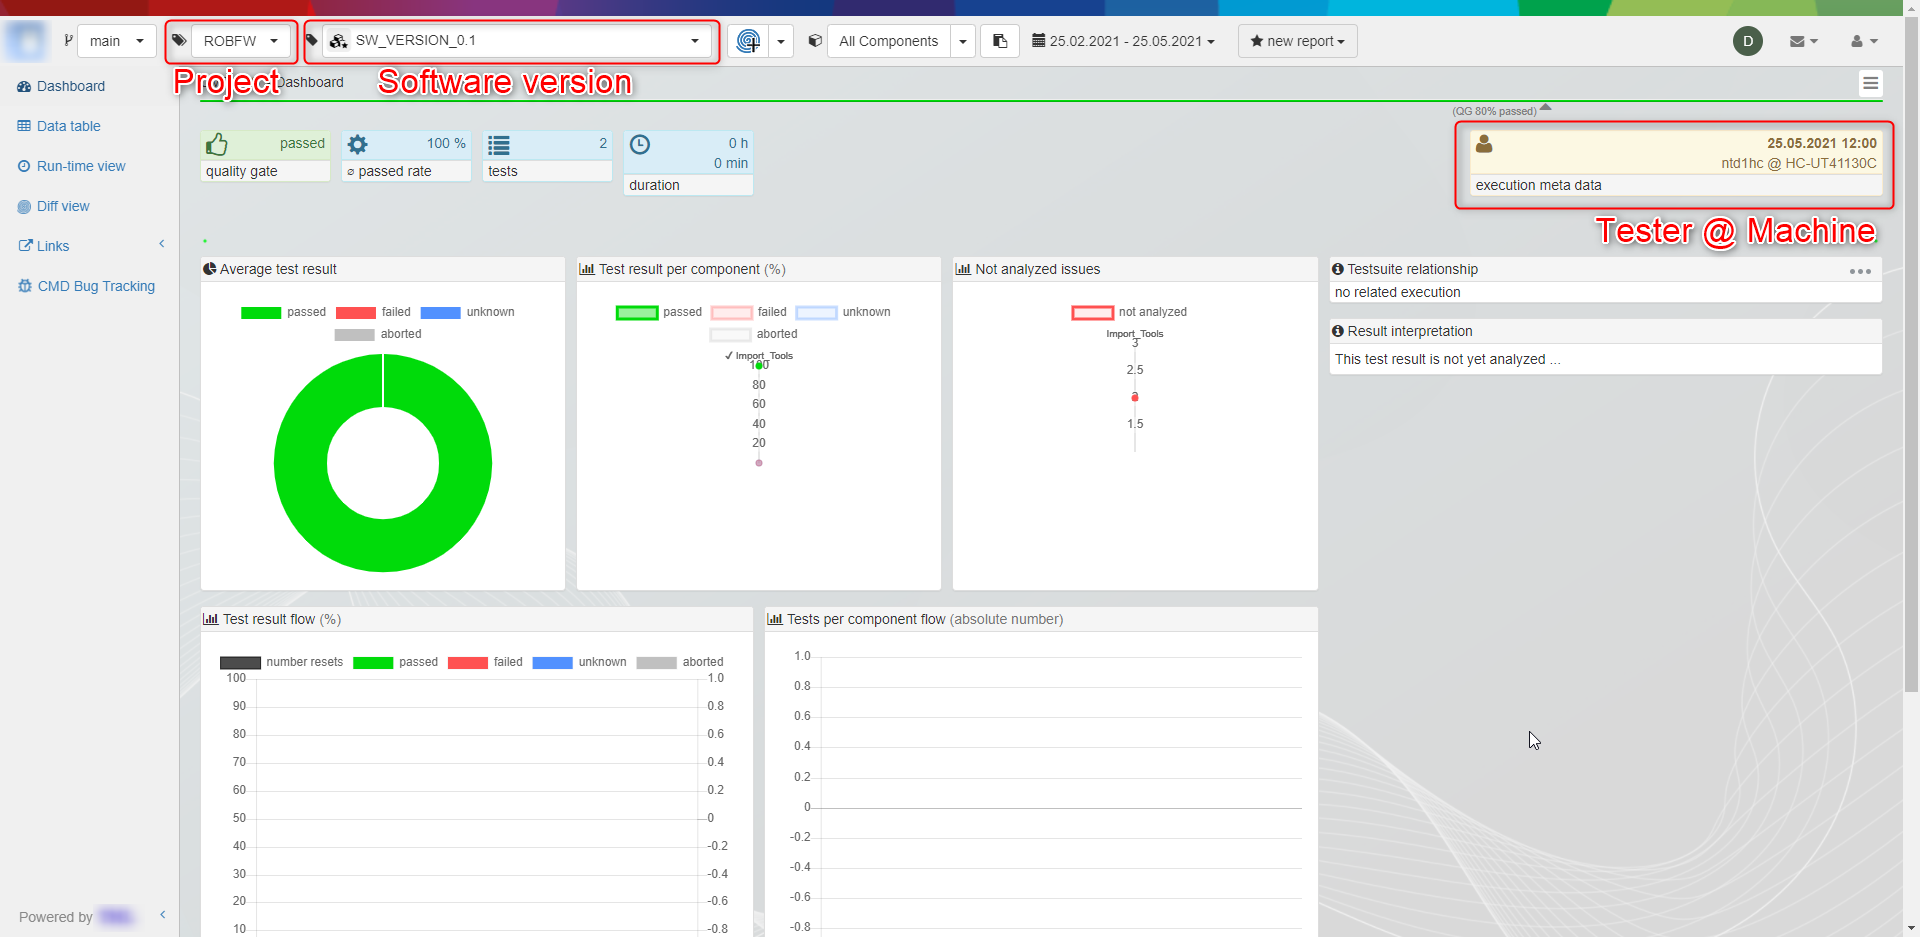
\includegraphics[width=1\linewidth]{./pictures/Dashboard.png}
  \caption{Dashboard view}
\end{figure}

Suite/File metadata and test case information:

\begin{figure}[h!]
  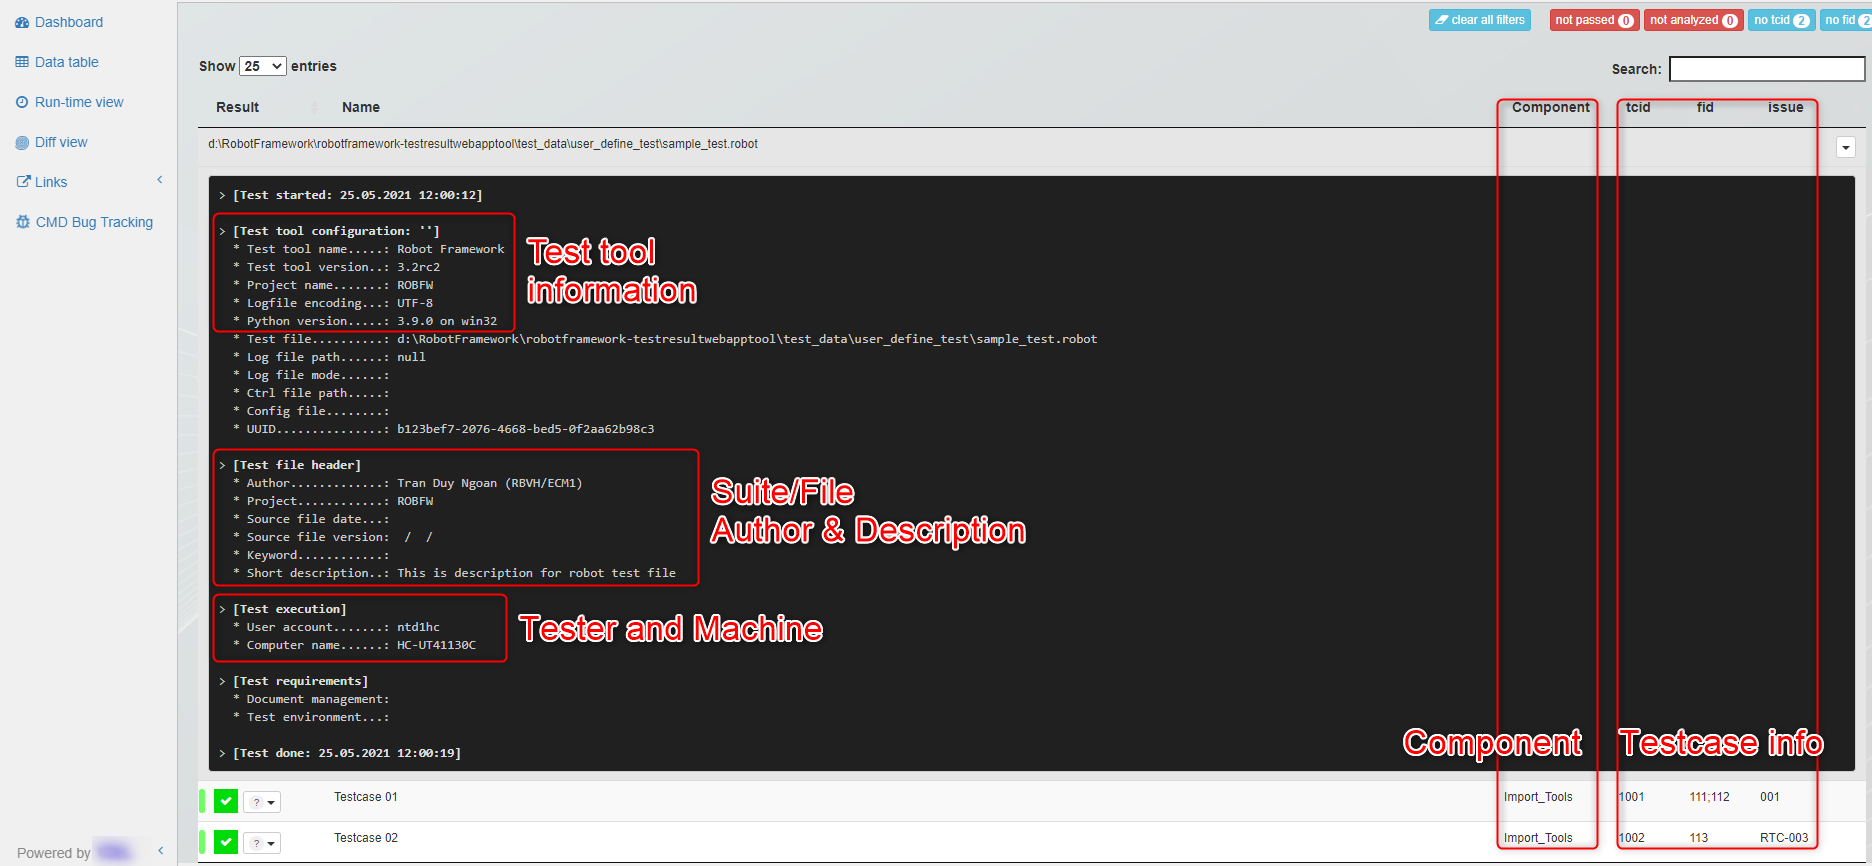
\includegraphics[width=1\linewidth]{./pictures/Datatable.png}
  \caption{Datatable view}
\end{figure}